%%%%%%%%%%%%%%%%%%%%%%%%%%%%%%%%%%%%%%%%%
% Plasmati Graduate CV
% LaTeX Template
% Version 1.0 (24/3/13)
%
% This template has been downloaded from:
% http://www.LaTeXTemplates.com
%
% Original author:
% Alessandro Plasmati (alessandro.plasmati@gmail.com)
%
% License:
% CC BY-NC-SA 3.0 (http://creativecommons.org/licenses/by-nc-sa/3.0/)
%
% Important note:
% This template needs to be compiled with XeLaTeX.
% The main document font is called Fontin and can be downloaded for free
% from here: http://www.exljbris.com/fontin.html
%
%%%%%%%%%%%%%%%%%%%%%%%%%%%%%%%%%%%%%%%%%

%----------------------------------------------------------------------------------------
%	PACKAGES AND OTHER DOCUMENT CONFIGURATIONS
%----------------------------------------------------------------------------------------

\documentclass[a4paper,10pt]{article} % Default font size and paper size

\usepackage{fontspec} % For loading fonts
\defaultfontfeatures{Mapping=tex-text}
\setmainfont[SmallCapsFont = Fontin SmallCaps]{Fontin} % Main document font

\usepackage{xunicode,xltxtra,url,parskip} % Formatting packages

\usepackage[usenames,dvipsnames]{xcolor} % Required for specifying custom colors
\usepackage[vmargin=1.5cm, hmargin=3cm]{geometry}
%\usepackage[big]{layaureo} % Margin formatting of the A4 page, an alternative to layaureo can be\usepackage{fullpage}
% To reduce the height of the top margin uncomment: \addtolength{\voffset}{-1.3cm}

\usepackage{hyperref} % Required for adding links	and customizing them
\definecolor{linkcolour}{rgb}{0,0.2,0.6} % Link color
\hypersetup{colorlinks,breaklinks,urlcolor=linkcolour,linkcolor=linkcolour} % Set link colors throughout the document

\usepackage{titlesec} % Used to customize the \section command
\titleformat{\section}{\Large\scshape\raggedright}{}{0em}{}[\titlerule] % Text formatting of sections
\titlespacing{\section}{0pt}{3pt}{3pt} % Spacing around sections

\usepackage{graphicx}
\usepackage{caption}
\usepackage{subcaption}
\usepackage{calc}
\usepackage{xcolor}
\usepackage{float}

\begin{document}

\pagestyle{empty} % Removes page numbering

\font\fb=''[cmr10]'' % Change the font of the \LaTeX command under the skills section

%----------------------------------------------------------------------------------------
%	NAME AND CONTACT INFORMATION
%----------------------------------------------------------------------------------------

\par{
\begin{figure}
\centering
\makebox[\textwidth][c]{
\begin{subfigure}{.5\textwidth}
  
  {\Huge Youness \textsc{DAFLI}}
\end{subfigure}%

\begin{subfigure}{.5\textwidth}
  \hspace{120pt}
  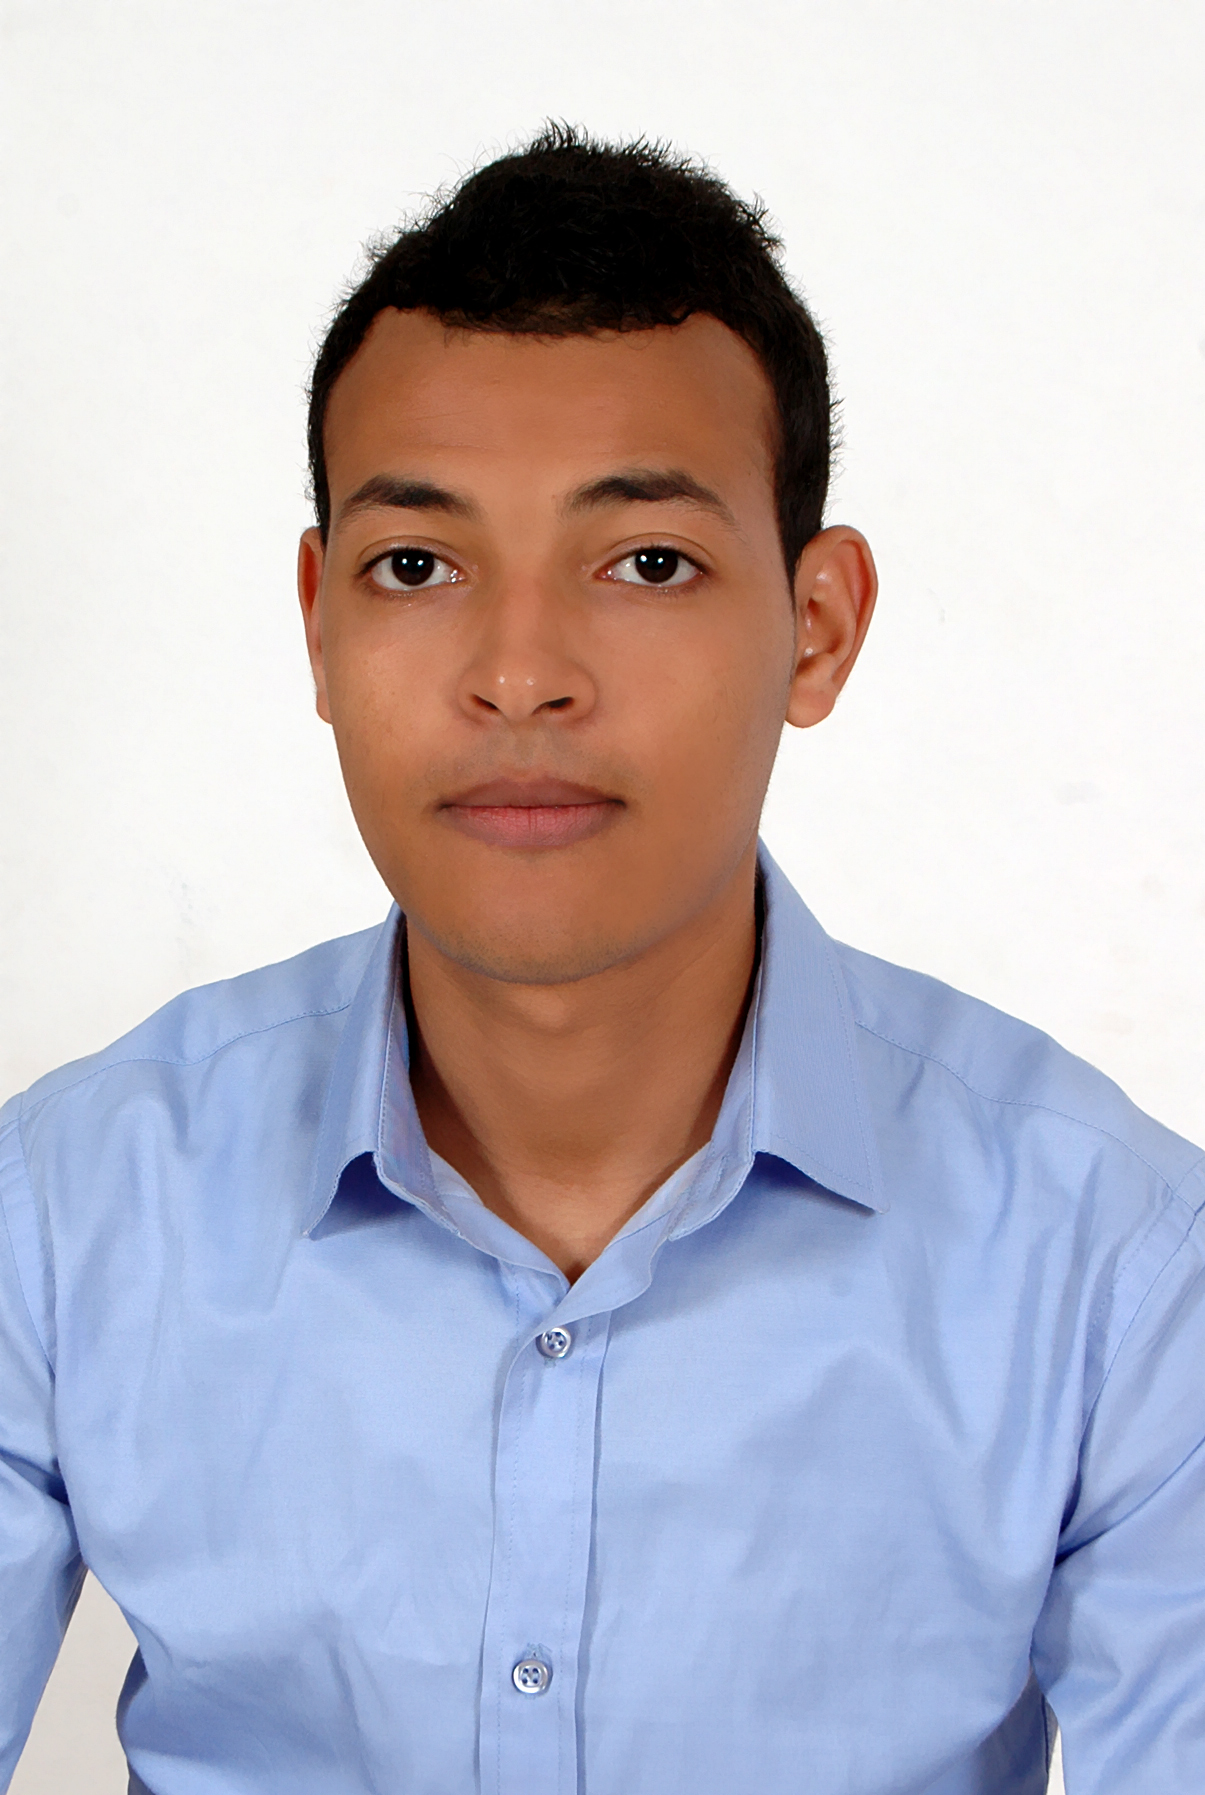
\includegraphics[scale=0.25]{photo.jpg}
\end{subfigure}
}
\end{figure}
}

\section{Données personnelles}

\begin{tabular}{rl}
\textsc{Age:} & 22 ans \\
\textsc{Adresse:} & Hay Saadiyine 1 Rue N0 20 Guelmim  \\
\textsc{Tél:} & 06.61.72.96.00\\
\textsc{e-mail:} & \href{mailto:youness.dafli@gmail.com}{youness.dafli@gmail.com}
\end{tabular}


\vspace{15pt}
\begin{quotation}
\textbf{Élève Ingénieur à la recherche d'un stage en développement logiciels}
\end{quotation}
\vspace{5pt}
              
%----------------------------------------------------------------------------------------
%	EDUCATION
%----------------------------------------------------------------------------------------

\section{Formation}

\begin{tabular}{r|p{13cm}}	
\textsc {2013-2014} & 
1\textsuperscript{ère} année, filière d'ingénieur en ``Génie logiciel et système d'informatique distribués''
\textbf{à l'École Normale Supérieure de l'Enseignement Technique (ENSET)}\\ \multicolumn{2}{c}{} \\

%------------------------------------------------

\textsc{2013} & Diplôme universitaire de technologie en `` Génie logiciel/Réseau'' \textbf{à l'École  Supérieure de Technologie ,Essaouira (EST)}.\\ \multicolumn{2}{c}{} \\

%------------------------------------------------

\textsc{2011} & Classe préparatoire option physique chimie et science de l'ingénieur (PCSI),
\textbf{lycée BAB SAHARA GUELMIM}.\\ \multicolumn{2}{c}{} \\

%------------------------------------------------

\textsc{2010} &  Baccalauréat, option science de la vie et de la terre \textbf{lycée BAB SAHARA GUELMIM}.
\end{tabular}

%----------------------------------------------------------------------------------------
%	SCHOLARSHIPS AND ADDITIONAL INFO
%----------------------------------------------------------------------------------------

\section{Connaissances professionnelles}

\begin{tabular}{rl}
\textsc{Programmation} & C, C++, JAVA ,PHP, Android, Assembleur \\

\textsc{Développement web} & HTML, XML, CSS, JavaScript \\

\textsc{Réseau} & Routage et adressage IP \\
\textsc{Systèmes d'exploitation} & Linux, Windows \\ 
\end{tabular}




%----------------------------------------------------------------------------------------
%	WORK EXPERIENCE 
%----------------------------------------------------------------------------------------

\section{Stages}

\begin{tabular}{r|p{11cm}}

\textsc{ 2013} & \emph{Deux mois au sein de l'Agence Urbaine de Guelmim-Es-Smara en service informatique}\\ 
& \footnotesize{création d'une application de gestion des stagiaire en java} \\
& \footnotesize{maintenance des ordinateurs / câblage réseau} \\
\multicolumn{2}{c}{} \\

%------------------------------------------------

\textsc{ 2012} & \emph{un mois au sein de Ministère des éqipements et de transport de Guelmim-Es-Smara en service informatique}\\ 
& \footnotesize{création d'une application de gestion de parc auto en php}.
\end{tabular}

%----------------------------------------------------------------------------------------
%	LANGUAGES
%----------------------------------------------------------------------------------------

\section{Langues}

\begin{tabular}{rl}
\textsc{Arabe:} & Langue maternelle\\

\textsc{Français:} & lue parlée et écrite \\

\textsc{Anglais:} & lue parlée et écrite \\
\end{tabular}

%----------------------------------------------------------------------------------------
%	INTERESTS AND ACTIVITIES
%----------------------------------------------------------------------------------------

\section{Centres d'intérêts }

Musique, Lecture, cinéma, Football \\

\end{document}
